\documentclass[12pt, a4paper]{article}

\usepackage[tbtags]{amsmath}
\usepackage{amssymb}
\usepackage{amsthm}

% \usepackage{tensor}

\usepackage{bm}
% \usepackage[italian]{babel}

% Section styling
\usepackage{titlesec}

\usepackage{mathrsfs}
\usepackage[dvipsnames]{xcolor}
% \usepackage[italian]{babel}

\usepackage{graphicx}
\usepackage{tikz}
\usepackage{caption}
\usepackage{subcaption}
\usepackage{mdframed}

\usepackage{enumerate}
\usepackage[LGR,T1]{fontenc}
\usepackage{hyperref}
\hypersetup{
	colorlinks=true,
	linkcolor=black,
	citecolor=black,
	filecolor=magenta,      
	urlcolor=blue,
	pdftitle={Matter},
	pdfpagemode=FullScreen,
}

\usepackage{csquotes}
\usepackage{booktabs}

\usepackage[hmargin = 3cm]{geometry}

% \usepackage[backend=biber, style=alphabetic, sorting=ynt]{biblatex}
% \addbibresource{Bibl.bib}

%\renewcommand\theequation{{\color{blue}\thesection.\arabic{equation}}}

\renewcommand{\Re}{\mathrm{Re}\,}
\renewcommand{\Im}{\mathrm{Im}\,}

\numberwithin{equation}{section}
\setlength{\parindent}{0 pt}

\pagestyle{plain}

\title{{\Huge\bf Simulation and data analysis} \\ 
    {\Huge\bf for an optics experiment about} \\ 
    {\Huge\bf spatial coherence} \bigskip \\ 

    {\Large Project for the exam of the course} \\ 
    {\Large "Scripting and programming laboratory}  \\ 
    {\Large for data analysis"}}

\author{Leonardo \textsc{Rossi}}
\date{}

\begin{document}
	\maketitle
    \newpage
	\tableofcontents
	\newpage
    
    \section{Introduction}

For this project, I wrote a simulation of an experiment and the code for analysis of the generated data, controlled by a GUI. The experiment concerns the (second order) 
statistics of a time independent speckle field , i.e. its spatial coherence. The statistical properties of the field can be controlled by a spatial filtering, 
and can be measured by interferometry, thus verifying the inverse proportionality relation between the width of the spatial spectrum and the correlation 
length predicted by the Wiener-Khintchine theorem. \\

% In this document I will focus on the physics of the experiment, the main results obtained from the simulation and their interpretation, while I will review the 
% characteristics of the code in a separated jupyter notebook.

\subsection{Set-up}

The arrangement of optical components in the main part of the experiment is as follows.

\begin{figure}[!ht]
    \centering
    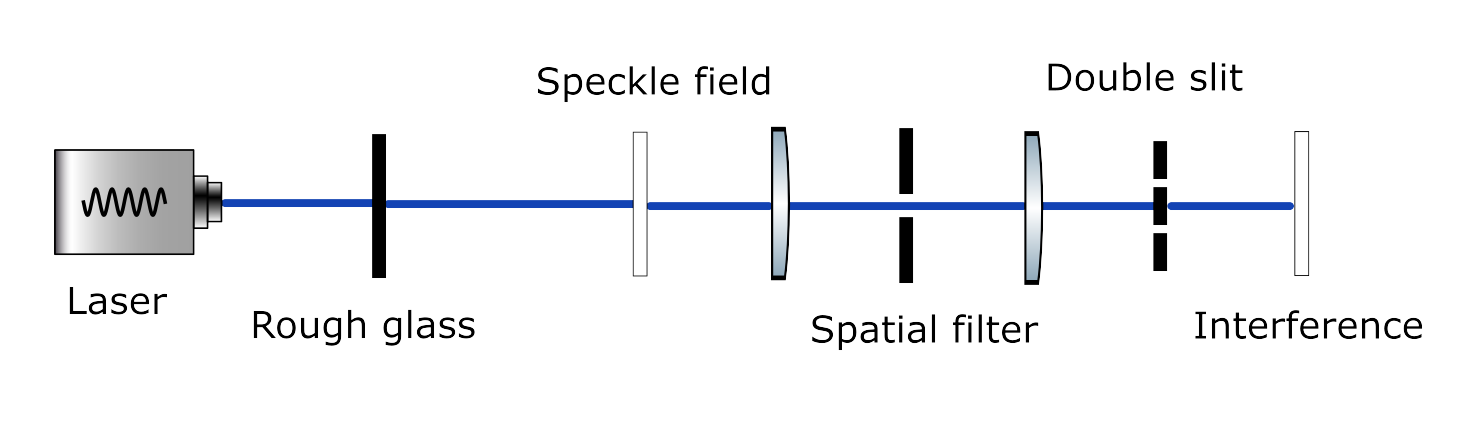
\includegraphics[width = .9\textwidth]{Img/setup.png}
    \caption{Set-up}
\end{figure}

The laser beam is assumed to have been previously expanded, filtered and collimated. The speckle field is produced by a rough glass surface, and is subsequently 
spatially filtered by a $4f$ set-up with a rectangular slit. Before filtering, the field already has a nonzero correlation length $\delta$ given by the Van Cittert-Zernike 
relation $\delta = z\lambda / D$ (where $z$ is the longitudinal propagation distance, $\lambda$ the wavelength and $D$ the diameter of the source, i.e. the collimated 
beam), which however is assumed to be negligible in comparison with the correlation induced by the filtering. \\

After filtering, the field has a (field) correlation function which is given by the Fourier transform of the filtered spectrum (Wiener-Khintchine theorem), 
which is

\begin{equation} \label{rect-corr}
    \gamma(s) = \mathrm{sinc}\,\left( \frac{\pi bs}{\lambda f} \right)
\end{equation}

for a rectangular filtering slit of width $b$ (here $f$ is the focal length of the lenses used for the filter). \\

This correlation function can be measured by Young interferometry: if the filtered field is probed by a double slit with separation $s$, one has the relation 

\begin{equation}
    \mathcal V = |\gamma(s)|,
\end{equation}

where $\mathcal V$ is the visibility, or contrast, of the interference pattern (the pattern is supposed to be averaged over an ensemble of speckle fields 
in order to capture the statistics). Once obtained the absolute value of $\gamma(s)$, the phase (which is always a $\pm 1$) can be inferred by the form of the 
pattern: if it has a central maximum, the phase is $+1$ (i.e., the two slits are on average in phase), while if it has a central minimum the phase is $-1$ 
(the two slits are out of phase). \\

By measuring the correlation function for different filtering widths one obtains the relation between correlation length and spectrum width.

\subsection{Simulation}

For simplicity, the simulation is done with $1$D instead of $2$D fields. The simulation also easily allows to filter the speckle field spectrum not only with 
a rectangular shape but e.g. with a gaussian shape, and it therefore showcases directly the Fourier transform relation given by the Wiener-Khintchine theorem. \\

Otherwise, the simulation closely follows the outline traced above: in the first part, a certain number ($\approx 200$) of $1$D speckle fields is generated 
and stored as csv files; in a second part, the  files are read and each one is fast-Fourier transformed, filtered, transformed back and used to generate an 
interference pattern. The patterns are then averaged over the ensemble, and the resulting averaged pattern is again stored as a csv. Finally, the patterns can 
be read and analyzed. \\


    \newpage
    \section{Review of the physics}

\subsection{Speckle fields} \label{speckles}

A "speckle field" is an optical field with a random pattern of constructive and destructive interference, which gives rise to little dots of lights called "speckles". 
A speckle field can be studied statistically, usually only considering first- and second-order statistics, i.e. the intensity distribution and the two-point 
correlation function. \\

The intensity correlation function of a speckle field with intensity $I(\bm x) \propto \langle |\bm E(\bm x)|^2 \rangle$, and its 
normalized version, are given by (assuming that they only depend on the separation between the two points)

\begin{equation}
    G(\bm s) = \langle I(\bm x)I(\bm x + \bm s) \rangle, \qquad g(\bm s) = \frac{G(\bm s)}{\langle I(\bm x)^2 \rangle}.
\end{equation}

$\langle \ \rangle$ denotes the average over an ensemble of fields. The intensity correlation function can be computed directly from the measured intensity. 
It characterizes the average size of the speckles, but it doesn't contain any information about the phase relation between two points. \\

By contrast, the field correlation function

\begin{equation}
    \Gamma(\bm s) = \langle \bm E(\bm x)^* \cdot \bm E(\bm x + \bm s)\rangle, \qquad \gamma(\bm s) = \frac{\Gamma(\bm s)}{\langle |\bm E(\bm x)|^2 \rangle}
\end{equation}

also contains the information about the phase relation, but it cannot be computed from a direct measurement of the field. Instead, it is necessary to use 
interferometry to obtain the necessary information about the average phase relation. 

\subsection{Measuring the field correlation function} \label{meas_corr}

Consider a double slit, neglecting for now the finite slit width effects, probing a $1$D speckle field. The far-field interference pattern is, for a slit 
separation $s$,

\begin{equation} \label{int_field}
    E_{\text{screen}}(y) = E\left(-\frac s2\right)\frac{e^{ikr_1}}{r_1} + E\left(\frac s2\right)\frac{e^{ikr_2}}{r_2},
\end{equation}

where $k = 2\pi/\lambda$ and $r_{1, 2}$ is the distance of the point on the screen $y$ from the two slits. The approximation to first order
$r_2 - r_1 = \sqrt{z^2 + (y - s/2)^2} - \sqrt{z^2 + (y + s/2)^2} \approx ys/2z$ is valid in the far-field regime ($z$ is the longitudinal propagation distance). 
Going over to the averaged intensity, 

\begin{equation}
    \langle |E_{\text{screen}}(y)|^2 \rangle = \frac 2{z^2}\Gamma(0) + \frac 2{z^2} \Re \left\{ \left\langle E\left(-\frac s2\right)^*E\left(\frac s2\right) \right\rangle  \exp\left( \frac{2\pi}{\lambda z} ys \right) \right\},
\end{equation}

where $\Gamma(0) = \langle |E(-s/2)|^2 \rangle =  \langle |E(s/2)|^2 \rangle$ is the average intensity of the speckle field. In the expression there appears the field correlation 
function $\Gamma(s) = |\Gamma(s)|e^{i\phi(s)}$. Therefore, modulo a $z^2$ factor,

\begin{equation} \label{part_cor_patt}
    \langle |E_{\text{screen}}(y)|^2 \rangle = 2 \, \Gamma(0) + 2 \, |\Gamma(s)| \cos\left[ \frac{2\pi}{\lambda z} sy + \phi(s) \right].
\end{equation}

The maximum intensity $I_{\text{max}}$ is attained when the cosine is $+1$, the minimum $I_{\text{min}}$ when the cosine is $-1$. Therefore 

\begin{equation}\label{vis_formula}
    \mathcal V = \frac{I_{\text{max}} - I_{\text{min}}}{I_{\text{max}} + I_{\text{min}}} = \frac{|\Gamma(s)|}{\Gamma(0)} = |\gamma(s)|.
\end{equation}

Finally, from the expression \eqref{part_cor_patt} it can be seen that the phase $\phi(s)$ of the correlation function determines the value of the pattern when 
$y = 0$. Thus, if $\langle |E_{\text{screen}}(0)|^2 \rangle = I_{\text{min}}$, then $\phi(s) = \pi$ and $e^{i\phi(s)} = -1$; if 
$\langle |E_{\text{screen}}(0)|^2 \rangle = I_{\text{max}}$, then $\phi(s) = 0$ and $e^{i\phi(s)} = +1$.

\subsection{Finite slit width effects}

In practice, the slits have a finite width (in the simulation it is of $a = 1 \, \mathrm{mm}$), and therefore the interference pattern is modulated by a certain 
profile. In the case of coherent light, the profile is a $\mathrm{sinc}$ function (the diffraction pattern from a single slit), but in the case of partially 
coherent light the profile is more complicated. The equation \eqref{int_field} becomes, taking into accout the finite width,

\begin{equation}
    E_{\text{screen}}(y) = \int_{-s/2-a/2}^{-s/2 + a/2} \mathrm dx \, E(x)\frac{e^{ikr(x)}}{r(x)} + \int_{s/2-a/2}^{s/2 + a/2} \mathrm dx \, E(x)\frac{e^{ikr(x)}}{r(x)},
\end{equation}

where $r(x) = \sqrt{z^2 + (y - x)^2}$. Without going over the whole calculation, the resulting pattern is, modulo a $z^2$ factor, and 
neglecting the partial coherence of the field over a single slit,

\begin{equation} \label{theopatt}
    \langle |E_{\text{screen}}(y)|^2 \rangle = 2a^2 \Gamma(0) \, \mathrm{sinc}  \left( \frac{\pi a y}{\lambda z} \right)^2 \left[ 1 + |\gamma(s)| \cos\left( \frac{2\pi}{\lambda z}sy +\phi(s) \right) \right]
\end{equation}

Actually, there are also the effects due to the partial coherence of the field over the span of a single slit; in the code, I accounted for those effects by 
inserting a corrective multiplicative constant in the amplitude (this correction is only empirically justified).

\subsection{Computing the field correlation function} \label{comp_corr}

The spatial filtering of the speckle field determines its second order statistics by the Wiener-Khintchine theorem, which states that the two-point correlation 
function is the fourier transform of the spectral density (which is proportional to the field in the focal plane of the spatial filter). Therefore, if $b$ denotes 
the width of the filtering slit, and assuming an initially $\delta$-correlated field (so that its spectral density is a constant), it is easy to obtain eqn. 
\eqref{rect-corr}. \\

The software will also allow the option of a gaussian filtering. In that case, the field correlation function in the double slit plane would be 

\begin{equation}
    \gamma(s) = \exp\left[-\left(\frac{\pi bs}{\lambda f}\right)^2\right].
\end{equation}


	\newpage
	\section{Results from the simulation}

% \subsection{Overview of the interface}

The simulation, as mentioned above, is articulated in three steps, managed by different windows of the GUI. The first is the generation of the speckle fields, 
the second is the spatial filtering together with caculation of the interference patterns using the resulting filtered speckle fileds, the third is the analysis of 
the patterns and the calculation of the correlation function.

% Maybe add some figures here, illustrating the GUI? Or keep that for the notebook?

% \subsection{Generation of the speckle fields} keep this for the notebook?

\subsection{Interference patterns}

The interference patterns produced look like figure \ref{patt}. In the figure, the modulating function of eqn. \eqref{theopatt} is also shown. Since this 
function is calculated neglecting the effects of partial coherence over each individual slit, the actual pattern has a lower intensity. \\

There are three main effects which in principle have to be taken into account, as can be seen in the figure: 
the modulation of the cosine (due to the finite width of the slits), the loss of visibility (due to the partial coherence between the field amplitudes at the two slits) 
and, as noted above, 
an overall reduction of the intensity if compared with coherent light (due to the partial coherence over the two individual slits). This last feature is accounted 
for by inserting a multiplicative constant as an additional parameter in the fit.
\begin{figure}[!ht]
    \centering
    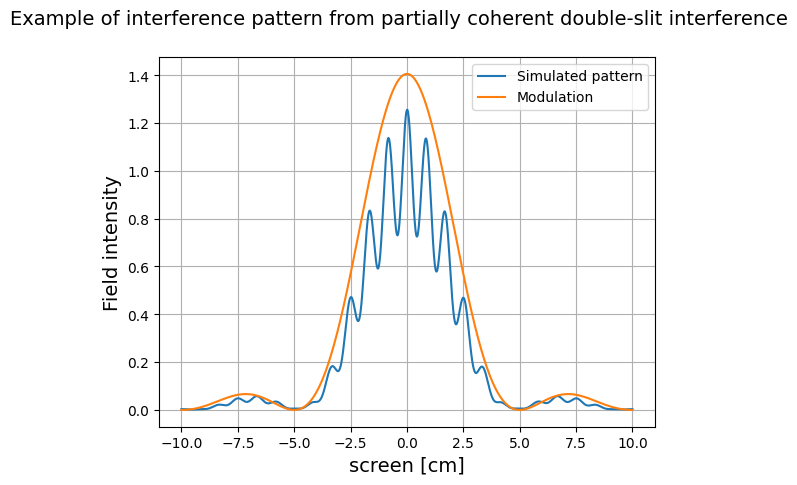
\includegraphics[width = .8\textwidth]{Img/output.png}
    \caption{Typical interference pattern}
    \label{patt}
\end{figure}

\subsection{Data analysis}

The interface for data analysis allows to automatically compute the visibility of each interference pattern (previously generated and stored as csv files) as 
a function of either the width of the spectral density after the spatial filtering, or the separation between the slits. In the latter case, the resulting 
function is exactly the absolute value of the normalized field correlation function, as per eqn. \eqref{vis_formula}: this allows to calculate the correlation 
length $\Delta l$ as the FWHM (or another width measure) of the correlation function. The dependence on the spectral density width $\Delta k$ allows then to 
verify the inverse proportionality between $\Delta l$ and $\Delta k$. \\

The automatic analysis of all the interference patterns is carried out by first dividing each one by the modulating function, suitably normalized, in order 
to obtain a nearly (co)sinusoidal pattern (like in figure \ref{data_an_2}); the visibility can then be calculated using eqn. \eqref{vis_formula}. 
It is also possible to consider an individual pattern at a time: in this case, the interface allows to choose the initial parameters in order to perform a 
fit of both the upper and lower profile of the interference pattern (the local maxima of the pattern belong to the upper profile and the local minima belong 
to the lower pattern). This is shown in figures \ref{data_an_1} and \ref{data_an_2}

\begin{figure}[!ht]
    \centering
    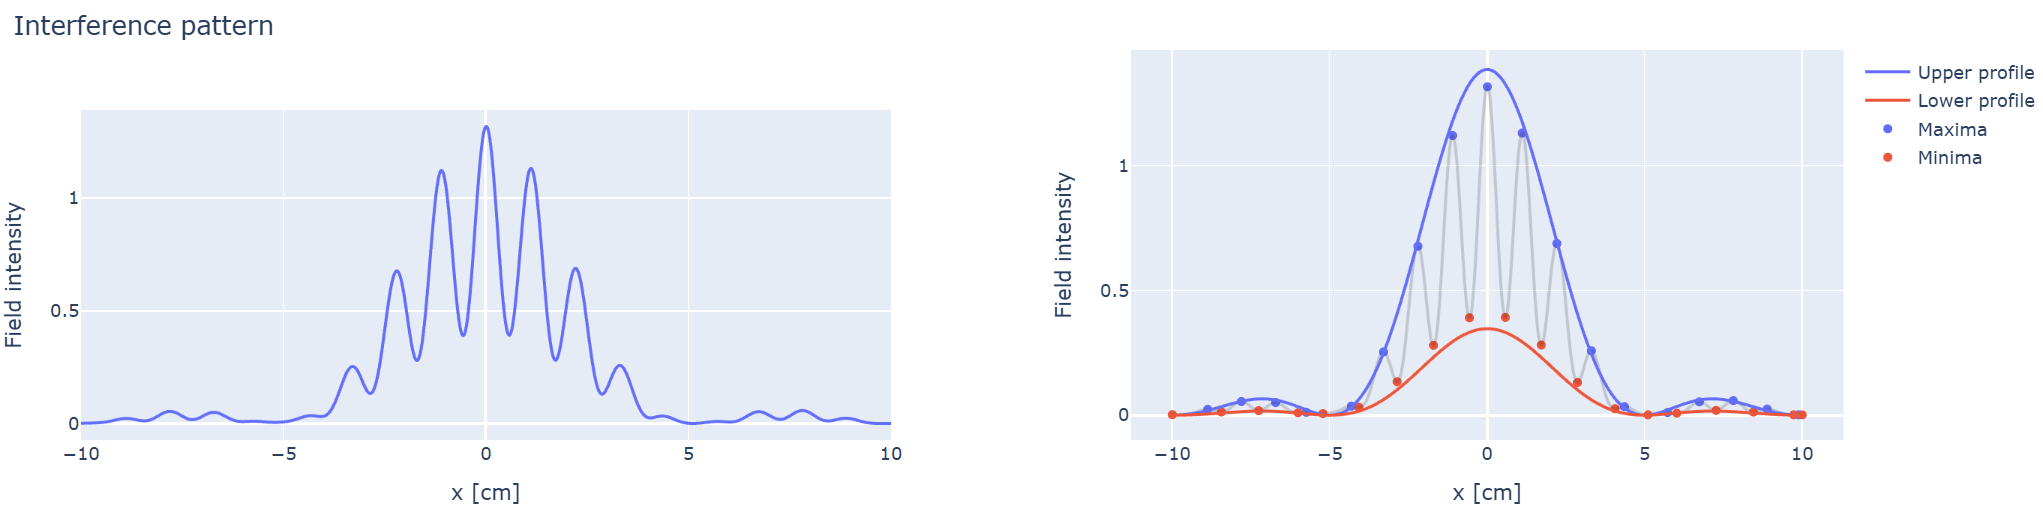
\includegraphics[width = \textwidth]{Img/an_11.png}
    \caption{Data analysis interface}
    \label{data_an_1}
\end{figure}

\begin{figure}[!ht]
    \centering
    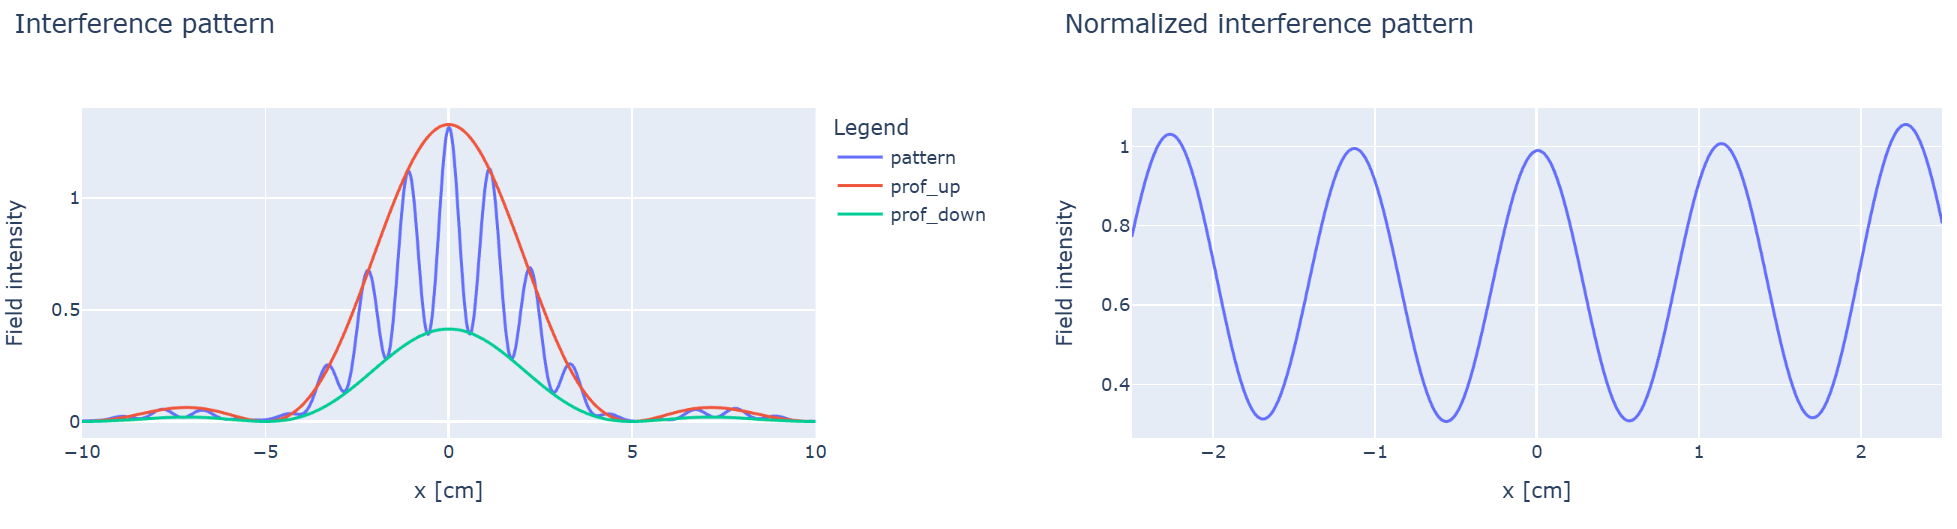
\includegraphics[width = \textwidth]{Img/an_22.png}
    \caption{Data analysis interface}
    \label{data_an_2}
\end{figure}



\end{document}